\documentclass[11pt]{article}

% ---------- Page setup ----------
\usepackage[margin=1in]{geometry}
\usepackage{lmodern}
\renewcommand{\familydefault}{\sfdefault}

% ---------- Packages ----------
\usepackage{microtype}
\usepackage{float}
\usepackage{xcolor}
\usepackage{titlesec}
\usepackage{tcolorbox}
\usepackage{hyperref}
\usepackage{graphicx}
\usepackage{caption}

% ---------- Colors ----------
\definecolor{main}{HTML}{1F4E79}
\definecolor{light}{HTML}{F5F7FA}

% ---------- Section style ----------
\titleformat{\section}
{\Large\bfseries\color{main}}
{}
{0em}
{}

% ---------- Box style ----------
\tcbset{
colback=light,
colframe=main,
boxrule=0.5pt,
arc=4pt,
left=8pt,
right=8pt,
top=6pt,
bottom=6pt
}

% ---------- Title ----------
\title{\textbf{MongoDB Sharding Hands-On Report}}
\author{}
\date{}

\begin{document}

\maketitle

\section*{Sharding Key and Sharding Strategy}

What is a sharding key? Is the choice of a sharding key directly dependent of the 
sharding strategy? Explain and give examples.



\begin{tcolorbox}

A sharding key is the attribute inside each document that MongoDB uses to determine how documents are partitioned across shards in a distributed cluster. The value of this key determines which chunk a document belongs to and how which shard will store it. In the exercises performed, the field \texttt{state} was used as the sharding key when creating collections such as \texttt{cities1} and \texttt{cities3}. This means MongoDB used the value of the state field to determine where documents should be placed in the cluster.

The choice of that sharding key definitely depends on the sharding strategy we want to use. For example, if we’re using range (or interval) sharding, we divide the data into continuous ranges of the key. If we use hash sharding, we hash the key so the data is spread out more evenly. In other words, the sharding key is the field we use to decide how to break data into chunks, and the strategy (like interval or hash) is how we actually do that breaking.

\end{tcolorbox}

The sh.status() output shows that the collection cities3 uses the field state as the sharding key. Tag ranges were defined so that documents with state CA are associated with shard1, NY with shard2, and other states with shard3. This illustrates how the shard key determines how documents are partitioned and how tag-based sharding can control where specific ranges of the key are stored.

\begin{center}
    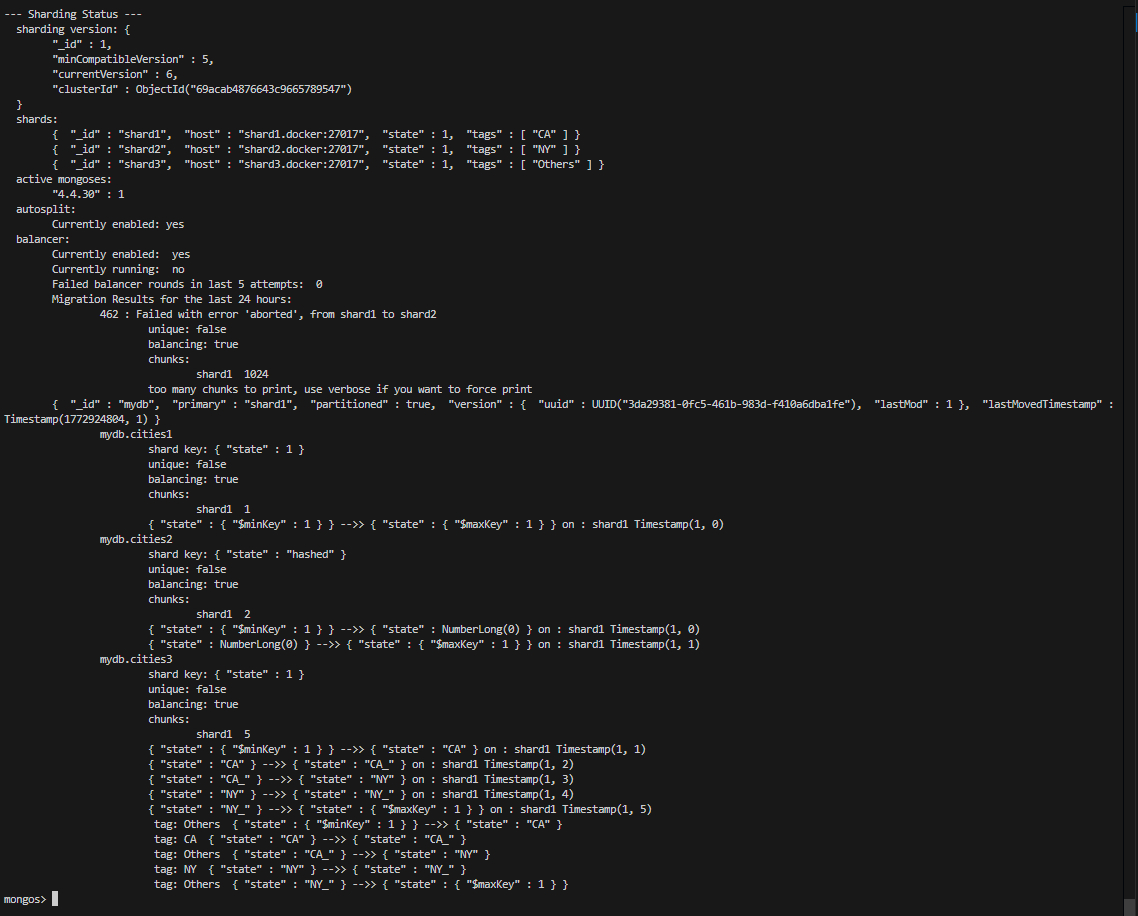
\includegraphics[width=0.8\textwidth]{Captura de pantalla 2026-03-07 194806.png}
    \captionof{figure}{Sharding configuration with tag-based ranges applied.}
    \label{fig:tag_sharding}
\end{center}






\section*{Interval Sharding Strategy}

Explain how does apparently mongodb choses the number of intervals used to shard a 
collection in the Interval oriented strategy? In which situations would such a strategy be 
well adapted for sharding a collection?  

\begin{tcolorbox}

In the interval (or range) sharding strategy, MongoDB starts by dividing the entire range of your sharding key into just a few chunks. Initially, you might see only one or two intervals (or chunks) covering the entire range of the key.

As you add more data, MongoDB automatically monitors the size of these chunks. When a chunk gets too big—typically around 64 MB of data—it splits that chunk into smaller intervals. Over time, as your data grows, MongoDB keeps splitting chunks to keep them evenly sized.

In other words: At the start, you just have a few big chunks. As data grows, MongoDB automatically splits them into more and more chunks.

This strategy is particularly well adapted for datasets where queries frequently target ranges of ordered values. Examples include time-based records, geographical attributes, or numeric identifiers where queries may request intervals of values. In such situations, range sharding allows MongoDB to route queries only to the shards containing the relevant intervals, improving query efficiency.

\end{tcolorbox}

The sh.status() output indicates that the collection cities1 was sharded using the field state with a range-based shard key. The system created one chunk spanning the full interval of the key (MinKey to MaxKey). Because only one shard existed at this stage, all documents remained on shard1. This shows how interval sharding organizes documents according to ordered ranges of the shard key.

\begin{figure}[ht]
    \centering
    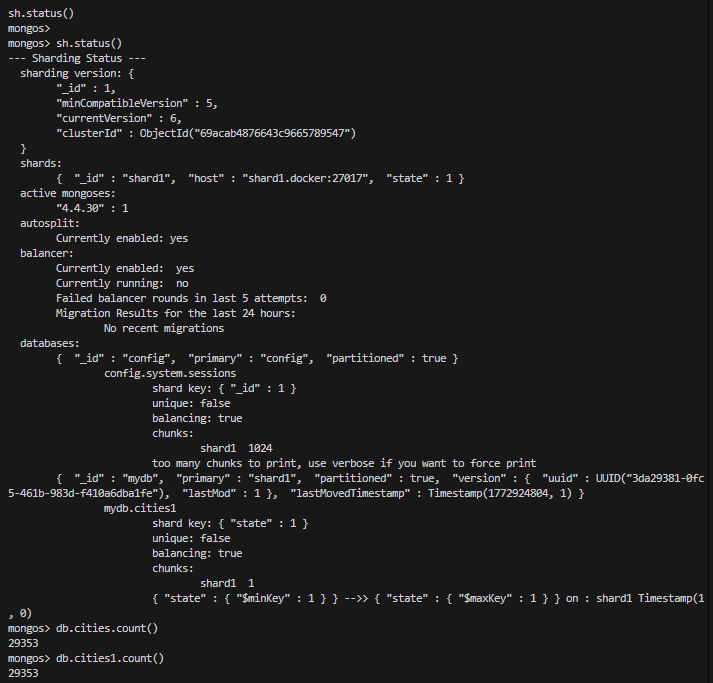
\includegraphics[width=0.8\textwidth]{Captura de pantalla 2026-03-07 202746.png}
    \caption{Interval-based sharding distribution for Cities1 collection.}
    \label{fig:interval_sharding}
\end{figure}







\section*{Hash-Based Sharding}

In which situations would the hash-based strategy be interesting for a collection to be 
sharded? 

\begin{tcolorbox}

Hash-based sharding distributes documents according to the hash value of the shard key rather than its natural ordering. By transforming the key through a hashing function, MongoDB spreads documents more evenly across shards and reduces the risk of data concentration on a single node. In the exercise this strategy was used when creating the \texttt{cities2} collection with the shard key defined as \texttt{state : "hashed"}.

This approach is particularly useful when the natural distribution of key values may create hotspots or when the application workload generates large volumes of inserts for similar key values. Hash-based sharding sacrifices some efficiency in range queries but provides a more balanced distribution of data across shards.This is especially interesting when you’re dealing with workloads where you don’t want any one shard to become a bottleneck.

\end{tcolorbox}

The sh.status() output indicates that the collection cities2 was sharded using a hashed shard key on the field state. MongoDB divides the hashed values of the key into chunks (MinKey → 0 and 0 → MaxKey), which distributes documents more uniformly than range-based sharding. This strategy reduces the risk of data hotspots and helps balance data distribution across shards.

\begin{figure}[ht]
    \centering
    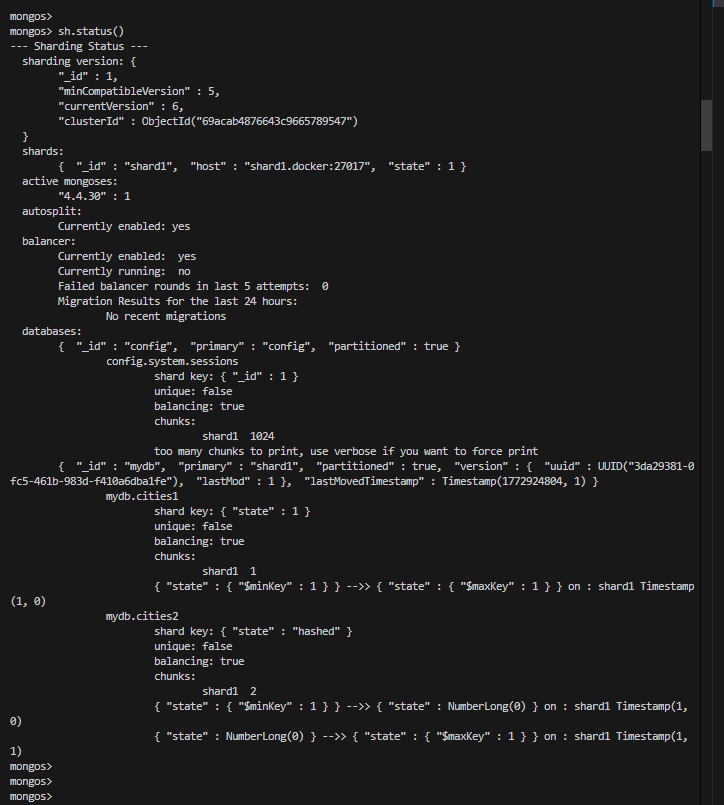
\includegraphics[width=0.8\textwidth]{image.png}
    \caption{Hash-based sharding distribution for Cities2 collection.}
    \label{fig:hash_sharding}
\end{figure}




\section*{Data Distribution and Cluster Behavior}

Which of the strategies interval or sharding would lead to a more balanced distribution 
of data across shards, interval, or hash?  

\begin{tcolorbox}

In general, hash-based sharding tends to produce a more balanced distribution of data across shards because the hashing process randomizes key values before assigning them to chunks. Range sharding may lead to uneven distributions if certain key ranges contain significantly more data than others. The experiment illustrated these behaviors by comparing collections using range and hash strategies, where the hashed collection created multiple chunks earlier in the process.

Direct access to shard servers can provide advantages for debugging or administrative inspection of data, but it bypasses the query router that normally manages request routing and data consistency. For this reason MongoDB generally recommends interacting with the cluster through the \texttt{mongos} router, which determines the correct shards to query and maintains the abstraction of a single logical database.

\end{tcolorbox}

\section*{Accessing Shards Directly vs. Using the Query Router}

What are the advantages and disadvantages of allowing access to shards directly through 
their server and not only through the query router?  

\begin{tcolorbox}

In a MongoDB sharded cluster, the query router (mongos) acts as a single point of contact for clients. When you query data, you send your requests to the query router, and it figures out which shards hold the relevant data, retrieves it, and merges the results. This makes life easier for most operations, as you don’t have to know where the data is stored.

However, there are pros and cons to accessing shards directly instead of going through the query router. One advantage is that direct access can be useful for debugging or performing maintenance tasks on a specific shard. On the downside, it introduces more complexity because you need to know exactly which shard to query, and you lose the convenience of automatic coordination. In general, the query router is recommended for everyday operations, while direct access is more of an advanced administrative tool.

\end{tcolorbox}

\section*{Tag-Based Sharding and Cluster Evolution}

Give an example of situation where tag based sharding would be an interesting option?  
What happens when a new shard is added to a cluster containing already other shards 
with data? 

\begin{tcolorbox}

Tag-based sharding allows administrators to associate ranges of shard key values with specific shards. In the exercise, tags such as \texttt{CA}, \texttt{NY}, and \texttt{Others} were assigned to shards and corresponding key ranges were defined for the \texttt{cities3} collection. This strategy can be useful when certain data must be stored in particular locations, such as geographic regions or regulatory zones.

When a new shard is added to a cluster, MongoDB's balancer automatically attempts to redistribute chunks from existing shards to the new node in order to maintain a balanced distribution of data. To evaluate whether sharding is beneficial compared to a centralized architecture, one can compare query performance, throughput, and scalability under increasing data volume or concurrent workloads. If the distributed cluster demonstrates improved performance or capacity, sharding becomes an effective solution for large-scale data management.

\end{tcolorbox}

An example of tag-based sharding was implemented in the experiment using the cities3 collection. In this configuration, ranges of the shard key state were associated with specific shard tags (CA, NY, and Others). This allowed documents corresponding to California and New York to be directed to particular shards while the remaining states were stored on another shard. The configuration can be observed in the sh.status() output shown in Figure 1.

\section*{Evaluating Sharding vs. a Centralized Database}

How would you test whether a sharded collection was an interesting solution in comparison to a centralized one?

\begin{tcolorbox}

To evaluate whether a sharded collection is a better solution than a centralized database, one would compare the performance and scalability of both configurations. A centralized database stores all the data on a single server, which can become a limitation when the dataset grows or when many users access the system simultaneously. In contrast, a sharded architecture distributes data across multiple servers, allowing the workload and storage to be shared among several machines.

In practice, this comparison could be tested by measuring query response time, throughput, and system load when running the same operations in both configurations. If the sharded system maintains stable performance while handling larger volumes of data or higher concurrency, then sharding can be considered a beneficial solution for the collection.

\end{tcolorbox}

\end{document}